% ! TEX root =../mechanics.tex

\part{空气动力学}
\chapter{基础知识}
流体力学认为物体的存在形态只有固态和液态两种
形态,区别在于固体可以通过产生有限的形变来承受
剪切应变.

流体力学作出的基本假设是连续介质假设.即把流体看
成连续不断,没有间隙,始终充满整个空间的连续介质.

控制体是在流场中一个有限封闭区域,这个区域就定义了
一个控制体.控制体可大可小,而这个控制体的封闭表面
就是控制面.换句话说,一个控制体对应着一个控制面.
控制体是固定在流场中的,流体从控制面流入.然后再流
出.当然,控制体也可以随着流体运动,而与周围的流体
没有交换.当控制体的体积趋于微元的控制体的时候,
称为微元体.
\begin{notice}
	微元的体积不能无限小,否则不满足连续介质假设了.
\end{notice}

流体具有压缩性,粘性,传热性等性质.
\begin{enumerate}
	\item 压缩性是指流体可以被压缩,压缩时流体的
	      体积发生变化.此时流体的密度一般也要发生变化.
	\item 粘性是指两层相邻速度不同的流体之间存在
	      着相互牵扯的力,称作粘性力或者内摩擦力.这个
	      力的大小与接触面法线的方向的速度梯度成正比.
	      \[
		      \tau=\mu \frac{\mathrm{d}u}{\mathrm{d}n}
	      \]
	\item 传热性是指流体沿某一方向存在温度梯度时,
	      热量就会从温度高的地方传向温度低的地方.
\end{enumerate}

流体的几个状态参数是压强$P$,温度$T$,密度$\rho$,
速度$\mathbf{V}$,焓值$h$等.这些参数都是关于
$x$,$y$,$z$,$t$的函数,也就是关于坐标和时间的函数.
其中坐标也是时间$t$的函数.

定常是指流体的状态参数和时间变化无关.

\section{流体模型}
\begin{enumerate}
	\item 理想流体 \\
	      不考虑流体的粘性作用的流体模型.
	\item 不可压流体 \\
	      不考虑流体压缩性的流体模型.不可压流体流场中
	      流体的密度是常数,即密度是定常的.
	\item 绝热流体 \\
	      不考虑流体传热性的流体模型,即与外界没有热交换.
\end{enumerate}

\section{量纲分析:白金汉\texorpdfstring{$\mathrm{\Pi}$}{Π}  定理(Dimensional Analysis: The BuckingHam PI Theorem)}
考虑一个给定形状的翼型在一定的攻角下,它受到的总空气动力是$R$。
在物理、直观的基础上,我们期望$R$取决于:
\begin{enumerate}
  \item 自由来流的速度$V_\infty$。
  \item 自由来流的密度$\rho_\infty$。
  \item 流体的黏度。我们已经知道剪切力$\tau$贡献了
    空气动力和空气动力矩,并且$\tau$正比于流体的流动
    的速度梯度。例如,如果给定速度梯度$\frac{\partial u}{\partial y}$,
    那么$\tau=\mu \frac{\partial u}{\partial y}$。这个常数的比例值$\mu$
    就是粘性系数。因此,我们用自由来流的粘性系数$\mu_\infty$来表示粘度对气动力和力矩
    的影响。
  \item 翼型的尺寸,以翼型的参考长度为代表。方便的参考长度是弦长$c$。
  \item 流体的可压性。可压性和遍及全流场的密度变化相关。相应的,可压性
    和流动过程中的声速相关。因此,我们用自由来流的声速$a_\infty$来表示
    可压性对气动力和力矩的影响。
\end{enumerate}

鉴于以上,在没有任何关于$R$变化的先验知识下,我们可以用常识写出:
\[
  R=f(\rho_\infty,V_\infty,c,\mu_\infty,a_\infty)
\]
上式就是一般的函数关系,对于计算$R$就不太实用。原则上,
我们可以将给定的翼型放到风洞中,倾斜到给定的攻角,然后
一次一个地
系统性地测量$R$由于$\rho_\infty$,$V_\infty$,$c$,$\mu_\infty$,
和$a_\infty$的变化而引起的变化。通过交叉绘制这样获得的大量数据,
我们就能提取出对于$R=f(\rho_\infty,V_\infty,c,\mu_\infty,a_\infty)$
的精确函数关系。然而,这肯定是一项艰苦的工作,而且就所需的大量风洞
实验的时间而言,这肯定是昂贵的。幸运的是,首先采用量纲分析的方法,
我们可以简化问题,大大减少我们的时间和精力。

这个方法先定义一组关于气动力和力矩的无量纲参数;这组参数将大大减少
出现在$R=f(\rho_\infty,V_\infty,c,\mu_\infty,a_\infty)$中自变量的
数量。

量纲分析基于一个很明显的事实,即对于真实物理世界中的方程,每一项都必须
具有相同的量纲。例如,如果
\[
  \Psi+\eta+\xi=\Phi
\]
是一个物理关系,那么$\Psi$,$\eta$,$\xi$和$\Phi$必须具有相同的
量纲。否则,我们就会把苹果和橘子加起来。上面那个方程可以通过
除以其中任何一个因子而变成无量纲的,比如$\Phi$:
\[
  \frac{\Psi}{\Phi}+\frac{\eta}{\Phi}+\frac{\xi}{\Phi}=1 
\]
这些思想在白金汉$\Pi$定理中有正式的体现。如下所示。
\begin{notice}
  {\bfseries 白金汉$\Pi$定理}

   设$K$表示描述物理变量所需的基本量纲数量。(在力学中,
   所有的物理变量都可以用质量,长度,时间的量纲来表示;
   因此,$K=3 $。)设$P_1$,$P_2$,$\cdots $,$P_N$表示
   在下述物理关系中的$N$个物理变量
   \[
     f_1(P_1,P_2, \ldots ,P_N)=0
   \]
   然后,上面的物理关系就可以重新表示为$(N-K)$个无量纲积($\Pi$积)的
   关系,
   \[
     f_2(\Pi_1,\Pi_2, \ldots ,\Pi_{N-K})=0
   \]
   在这些无量纲积中,每个$\Pi$积是一个有一组$K$个物理变量
   乘上一个其他物理变量的无量纲积。设$P_1$,$P_2$,$\cdots$,
   $P_K$是被选择的$K$个物理变量,那么:
   \begin{align*}
     \Pi_1&=f_3(P_1,P_2, \ldots ,P_K,P_{K+1})\\ 
     \Pi_2&=f_4(P_1,P_2, \ldots ,P_K,P_{K+2})\\ 
     \Pi_3&=f_5(P_1,P_2, \ldots ,P_K,P_{K+3})\\ 
     \cdots &\cdots \cdots \cdots \cdots \\ 
     \Pi_{N-K}&=f_5(P_1,P_2, \ldots ,P_K,P_N)
   \end{align*}
   重复变量的选择,$P_1$,$P_2$,$\cdots $,$P_K$应该包含用于这个问题
   的所有量纲。当然,这些相互独立的变量应当只在$\Pi$积中出现一次。
\end{notice}

回到,我们考虑的对于给定攻角和给定翼型的气动力和力矩的问题中,
方程
\[
  R=f(\rho_\infty,V_\infty,c,\mu_\infty,a_\infty)
\]
可以写成
\[
  g(R,\rho_\infty,V_\infty,c,\mu_\infty,a_\infty)=0
\]
的形式。根据白金汉$\Pi$定理,基本的量纲是
\begin{align*}
  m&=质量的量纲\\ 
  l&=长度的量纲\\ 
  t&=时间的量纲
\end{align*}
因此,$K=3 $。物理变量和他们的量纲是
\begin{align*}
  [R]&=mlt^{-2}\\ 
  [\rho_\infty]&=ml^{-3}\\ 
  [V_\infty]&=lt^{-1}\\ 
  [c]&=l\\ 
  [\mu_\infty]&=ml^{-1}t^{-1}\\ 
  [a_\infty]&=lt^{-1}
\end{align*}
因此,$N=6$。在上述,气动力$R$的量纲是通过牛顿第二定律获得的,
力=质量$\times$加速度;因此$[R]=mlt^{-2}$。$\mu_\infty$的量纲
是通过它的定义获得的,并且使用了牛顿第二定理。将$\rho_\infty$,
$V_\infty$和$c$作为任意选取$K$个物理变量中的几个。那么
\[
  g(R,\rho_\infty,V_\infty,c,\mu_\infty,a_\infty)=0
\]
可以用$N-K=6-3=3$个无量纲$\Pi$积来重新表示:
\[
  f_2(\Pi_1,P_2,P_3)=0
\]
这些$\Pi$积是:
\begin{align*}
  \Pi_1&=f_3(\rho_\infty,V_\infty,c,R)\\ 
  \Pi_2&=f_4(\rho_\infty,V_\infty,c,\mu_\infty)\\ 
  \Pi_3&=f_5(\rho_\infty,V_\infty,c,a_\infty)
\end{align*}
首先,集中注意在$\Pi_1$上,从上述方程组中的第一个,假定
\[
  \Pi_1=\rho_\infty ^d V_\infty ^b c^e R 
\]
$d$,$b$,$e$是需要找到的指数。在量纲上,上式就是
\[
  [\Pi_1]=(ml^{-3})^d(lt^{-1})^b(l)^e(mlt^{-2})
\]
因为$\Pi_1$是无量纲的,因此,上面方程的右边就必须是无量纲的。
这意味着量纲$m$的指数加起来必须是0,对于量纲$l$和$t$也是
一样的。因此
\begin{align*}
  对于m:& d+l&=0\\ 
  对于l:&-3d+b+e+1&=0\\ 
  对于t:&-b-2&=0
\end{align*}
解上述方程,我们可以得到$d=-1$,$b=-2$和$e=-2$。代入到方程
\[
  \Pi_1=\rho_\infty ^d V_\infty ^b c^e R 
\]
中,得到
\[
  \begin{split} 
    \Pi_1&=R \rho_\infty ^{-1} V_\infty ^{-2} c^{-2}\\ 
         &=\frac{R}{\rho_\infty V_\infty ^2 c^2}
  \end{split}
\]
物理量$\frac{R}{\rho_\infty V_\infty ^2 c^2}$是一个
无量纲的参数,其中$c^2$是一个面积,我们可以将$c^2$替换
为任何我们希望的参考面积(例如机翼的平面面积$S$),并且
$\Pi_1$将依然是无量纲的。更重要的是,我们可以将$\Pi_1$乘
一个纯粹的数量,并且它依然是无量纲的。因此,从上面的方程,
$\Pi_1$可以被定义为
\[
  \Pi_1=\frac{R}{\frac{1}{2}\rho_\infty V_\infty ^2 S}=\frac{R}{q_\infty S}
\]
因此,$\Pi_1$是气动力系数$C_R$。在上式中,$S$就是和给定翼型
有着密切关系的参考面积。

剩余的$\Pi$积可以按照相同的方法求出来。假设
\[
  \Pi_2=\rho_\infty V_\infty ^h c^i \mu_\infty ^j
\]
参考上述的分析,我们可以获得
\[
  [\Pi_2]=(ml^{-3})(lt^{-1})^h(l)^i(ml^{-1}t^{-1})^j
\]
因此,
\begin{align*}
  1+j&=0\\ 
  -3+h+i-j&=0\\ 
  -h-j&=0
\end{align*}
因此,$j=-1$,$h=1$,和$i=1$。代入到上式中就有
\[
  \Pi_2=\frac{\rho_\infty V_\infty c}{\mu_\infty}
\]
这个无量纲结合体被定义为雷诺数。雷诺数是在流动中物理测量的惯性力和
粘性力的比值,并且在流体力学中是最有力的参数之一。

再假设
\begin{align*}
  \Pi_3=V_\infty \rho_\infty ^k c^r a_\infty ^s \\ 
  [\Pi_3]=(lt^{-1})(ml^{-3})^k(l)^r(lt^{-1})^s 
\end{align*}
同样得到方程组
\[
  \begin{split}
    k&=0\\ 
    1-3k+r+s&=0\\ 
    -1-s&=0
  \end{split}
\]
因此,$k=0$,$s=-1$,$r=0$。代入到上式有,
\[
  \Pi_3=\frac{V_\infty}{a_\infty}
\]
这个无量纲量被定义为马赫数$M=\frac{V_\infty}{a_\infty}$。
马赫数是流动速度和声速的比值;它是研究气体动力的强有力
的参数。

无量纲分析的结果可以被写成如下
\begin{align*}
  f_2(\frac{R}{\frac{1}{2}\rho_\infty v_\infty ^2 S},
  \frac{\rho_\infty V_\infty c }{\mu_\infty },
  \frac{V_\infty }{a_\infty})=0\\ 
  f_2(C_R,Re,M_\infty)=0\\ 
  C_R=f_6(Re,M_\infty)
\end{align*}
这是一个重要的结果!在一开始,$R$被表示成有5个独立变量的
一般函数关系。然而,我们的量纲分析已经表示成:
\begin{enumerate}
  \item $R$可以被表示为无量纲气动力系数的项,
    $C_R=\frac{R}{\frac{1}{2}\rho_\infty V_\infty ^2 S }$。
  \item $C_R$只是Re和$M_\infty$的函数。 
\end{enumerate}
因此,通过用白金汉$\Pi$定理,可以减少不相互独立变量的数目,即
从5个变量减少成2个变量。现在,如果我们希望对一个给定的翼型在一个
固定的攻角下,做一系列风洞测试,我们只需要变化雷诺数和马赫数去获得
数据得到$R$的计算公式。通过很少的分析,我们就已经节约了很多努力和大量
的风洞时间。更重要的是,我们定义了两个控制流动的
无量纲参数,雷诺数和马赫数。它们叫做{\bfseries 相似参数(similarity 
parameters)}。因为升力和阻力都是总空气动力的分量,因此
\[
  C_L=f_7(Re,M_\infty)
\]
\[
  C_D=f_8(Re,M_\infty)
\]
更重要的是,这个关系对于气动力矩也成立,即
\[
  C_M=f_9(Re,M_\infty)
\]
请记住,上述关系是对于给定翼型在固定攻角下成立的。如果$\alpha$
是允许可变的,那么$C_L$,$C_D$,$C_M$都是依赖于变量$\alpha$的。
因此
\[
  C_L=f_{10}(Re,M_\infty,\alpha)
\]
\[
  C_D=f_{11}(Re,M_\infty,\alpha)
\]
\[
  C_M=f_{12}(Re,M_\infty,\alpha)
\]
上述方程的前提是假定翼型形状是给定的。大量的理论和实验
都聚焦在获取对于固定翼型形状的清晰的表达式,即上述方程。

\section{气动力和气动力矩}
\label{气动力和气动力矩}
气动力的来源主要有两部分,即:
\begin{enumerate}
	\item 作用在机翼表面的压强力。
	\item 作用在机翼表面的剪切力。
\end{enumerate}
无论机翼形状多么复杂,气动力和气动力矩总是
来源于上述两个方面。一般把垂直于机翼表面的
力称作{\bfseries 压强力(pressure stress)}。平行于机翼表面的
力称作{\bfseries 剪切力(shear stress)}。将压强力和剪切力
沿机翼表面积分,得到总空气动力$R$和总空气
动力矩$M$,并将总空气动力的作用点叫做{\bfseries 压心}。
如下图\ref{fig:airfoil force},将机翼远前方的气流速度记作$V_\infty$,
远离机翼的流体也叫做{\bfseries 自由来流(freestream)},因此,
$V_\infty$也叫做自由来流速度。

\begin{figure}[!ht]
	\centering
	% ! TEX root = ./introductory_thoughts.tex
\tikzset{every picture/.style={line width=0.75pt}} %set default line width to 0.75pt        

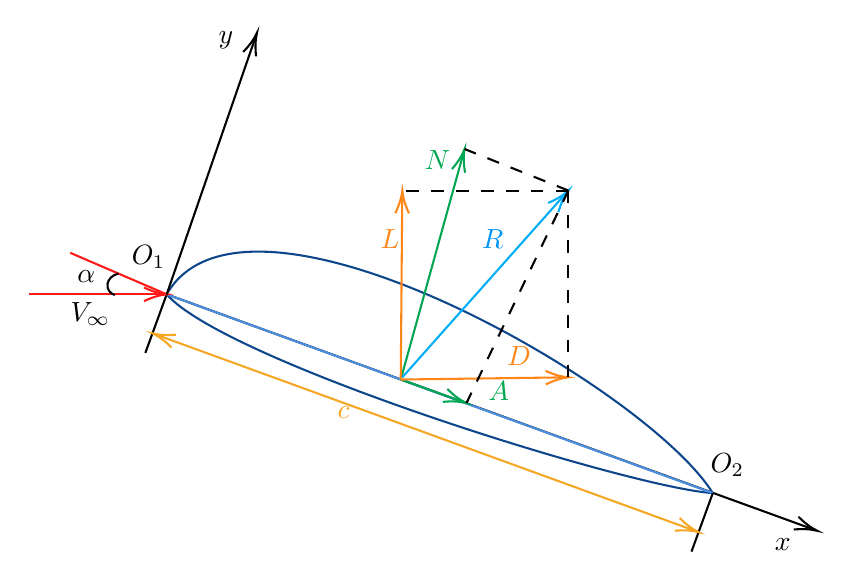
\begin{tikzpicture}[x=0.75pt,y=0.75pt,yscale=-1,xscale=1]
	%uncomment if require: \path (0,353); %set diagram left start at 0, and has height of 353

	%Straight Lines [id:da1842109967268275] 
	\draw    (186.47,136.04) -- (498.12,249.32) ;
	\draw [shift={(500,250)}, rotate = 199.97] [color={rgb, 255:red, 0; green, 0; blue, 0 }  ][line width=0.75]    (10.93,-3.29) .. controls (6.95,-1.4) and (3.31,-0.3) .. (0,0) .. controls (3.31,0.3) and (6.95,1.4) .. (10.93,3.29)   ;
	%Curve Lines [id:da035648358588663775] 
	\draw [color={rgb, 255:red, 14; green, 70; blue, 139 }  ,draw opacity=1 ]   (186.47,136.04) .. controls (224.32,69.81) and (417.44,180.11) .. (449.59,231.81) ;
	%Curve Lines [id:da2965896641352135] 
	\draw [color={rgb, 255:red, 14; green, 70; blue, 139 }  ,draw opacity=1 ]   (186.47,136.04) .. controls (214.79,168.5) and (409.77,229.25) .. (449.59,231.81) ;
	%Straight Lines [id:da05743983968805111] 
	\draw [color={rgb, 255:red, 74; green, 144; blue, 226 }  ,draw opacity=1 ]   (186.47,136.04) -- (449.59,231.81) ;
	%Straight Lines [id:da10439448052891231] 
	\draw    (449.59,231.81) -- (439.33,260) ;
	%Straight Lines [id:da788041337249308] 
	\draw    (186.47,136.04) -- (176.21,164.23) ;
	%Straight Lines [id:da7611175858700716] 
	\draw [color={rgb, 255:red, 245; green, 166; blue, 35 }  ,draw opacity=1 ]   (292.4,195.88) -- (440.87,249.92) ;
	\draw [shift={(442.75,250.6)}, rotate = 200] [color={rgb, 255:red, 245; green, 166; blue, 35 }  ,draw opacity=1 ][line width=0.75]    (10.93,-3.29) .. controls (6.95,-1.4) and (3.31,-0.3) .. (0,0) .. controls (3.31,0.3) and (6.95,1.4) .. (10.93,3.29)   ;
	%Straight Lines [id:da4556885360753773] 
	\draw [color={rgb, 255:red, 245; green, 166; blue, 35 }  ,draw opacity=1 ][fill={rgb, 255:red, 245; green, 166; blue, 35 }  ,fill opacity=1 ]   (292.4,195.88) -- (181.51,155.52) ;
	\draw [shift={(179.63,154.84)}, rotate = 20] [color={rgb, 255:red, 245; green, 166; blue, 35 }  ,draw opacity=1 ][line width=0.75]    (10.93,-3.29) .. controls (6.95,-1.4) and (3.31,-0.3) .. (0,0) .. controls (3.31,0.3) and (6.95,1.4) .. (10.93,3.29)   ;
	%Straight Lines [id:da3164870624705869] 
	\draw [color={rgb, 255:red, 0; green, 166; blue, 82 }  ,draw opacity=1 ]   (299.24,177.09) -- (329.47,67.96) ;
	\draw [shift={(330,66.04)}, rotate = 105.48] [color={rgb, 255:red, 0; green, 166; blue, 82 }  ,draw opacity=1 ][line width=0.75]    (10.93,-3.29) .. controls (6.95,-1.4) and (3.31,-0.3) .. (0,0) .. controls (3.31,0.3) and (6.95,1.4) .. (10.93,3.29)   ;
	%Straight Lines [id:da47805468728724976] 
	\draw [color={rgb, 255:red, 0; green, 166; blue, 82 }  ,draw opacity=1 ]   (299.24,177.09) -- (329.03,187.78) ;
	\draw [shift={(330.91,188.45)}, rotate = 199.74] [color={rgb, 255:red, 0; green, 166; blue, 82 }  ,draw opacity=1 ][line width=0.75]    (10.93,-3.29) .. controls (6.95,-1.4) and (3.31,-0.3) .. (0,0) .. controls (3.31,0.3) and (6.95,1.4) .. (10.93,3.29)   ;
	%Straight Lines [id:da9044725657133146] 
	\draw [color={rgb, 255:red, 255; green, 25; blue, 25 }  ,draw opacity=1 ]   (120,136.04) -- (184.47,136.04) ;
	\draw [shift={(186.47,136.04)}, rotate = 180.01] [color={rgb, 255:red, 255; green, 25; blue, 25 }  ,draw opacity=1 ][line width=0.75]    (10.93,-3.29) .. controls (6.95,-1.4) and (3.31,-0.3) .. (0,0) .. controls (3.31,0.3) and (6.95,1.4) .. (10.93,3.29)   ;
	%Straight Lines [id:da007233215583360764] 
	\draw [color={rgb, 255:red, 255; green, 134; blue, 24 }  ,draw opacity=1 ]   (299.24,177.09) -- (299.98,88.04) ;
	\draw [shift={(300,86.04)}, rotate = 90.48] [color={rgb, 255:red, 255; green, 134; blue, 24 }  ,draw opacity=1 ][line width=0.75]    (10.93,-3.29) .. controls (6.95,-1.4) and (3.31,-0.3) .. (0,0) .. controls (3.31,0.3) and (6.95,1.4) .. (10.93,3.29)   ;
	%Straight Lines [id:da3618051683565324] 
	\draw [color={rgb, 255:red, 255; green, 134; blue, 24 }  ,draw opacity=1 ]   (299.24,177.09) -- (378,176.06) ;
	\draw [shift={(380,176.04)}, rotate = 179.26] [color={rgb, 255:red, 255; green, 134; blue, 24 }  ,draw opacity=1 ][line width=0.75]    (10.93,-3.29) .. controls (6.95,-1.4) and (3.31,-0.3) .. (0,0) .. controls (3.31,0.3) and (6.95,1.4) .. (10.93,3.29)   ;
	%Straight Lines [id:da04699365108287412] 
	\draw [color={rgb, 255:red, 0; green, 174; blue, 247 }  ,draw opacity=1 ]   (300,176.04) -- (378.67,87.53) ;
	\draw [shift={(380,86.04)}, rotate = 131.63] [color={rgb, 255:red, 0; green, 174; blue, 247 }  ,draw opacity=1 ][line width=0.75]    (10.93,-3.29) .. controls (6.95,-1.4) and (3.31,-0.3) .. (0,0) .. controls (3.31,0.3) and (6.95,1.4) .. (10.93,3.29)   ;
	%Straight Lines [id:da6731669887886254] 
	\draw  [dash pattern={on 4.5pt off 4.5pt}]  (380,86.04) -- (300,86.04) ;
	%Straight Lines [id:da61043324884377] 
	\draw  [dash pattern={on 4.5pt off 4.5pt}]  (380,86.04) -- (380,176.04) ;
	%Straight Lines [id:da16658450416549608] 
	\draw  [dash pattern={on 4.5pt off 4.5pt}]  (380,86.04) -- (330,66.04) ;
	%Straight Lines [id:da03948089339816563] 
	\draw  [dash pattern={on 4.5pt off 4.5pt}]  (380,86.04) -- (330.91,188.45) ;
	%Straight Lines [id:da8326545905273048] 
	\draw [color={rgb, 255:red, 255; green, 25; blue, 25 }  ,draw opacity=1 ]   (140,116.04) -- (186.47,136.04) ;
	%Curve Lines [id:da294193336921325] 
	\draw    (163.24,126.04) .. controls (157.01,127.45) and (156.01,134.45) .. (161.51,136.45) ;
	%Straight Lines [id:da6512080695488691] 
	\draw    (186.47,136.04) -- (229.35,11.89) ;
	\draw [shift={(230,10)}, rotate = 109.05] [color={rgb, 255:red, 0; green, 0; blue, 0 }  ][line width=0.75]    (10.93,-3.29) .. controls (6.95,-1.4) and (3.31,-0.3) .. (0,0) .. controls (3.31,0.3) and (6.95,1.4) .. (10.93,3.29)   ;


	% Text Node
	\draw (210,8.07) node [anchor=north west][inner sep=0.75pt]    {$y$};
	% Text Node
	\draw (478,252.4) node [anchor=north west][inner sep=0.75pt]    {$x$};
	% Text Node
	\draw (267.33,188.73) node [anchor=north west][inner sep=0.75pt]  [color={rgb, 255:red, 245; green, 166; blue, 35 }  ,opacity=1 ]  {$c$};
	% Text Node
	\draw (142,123) node [anchor=north west][inner sep=0.75pt]    {$\alpha $};
	% Text Node
	\draw (168.07,111.32) node [anchor=north west][inner sep=0.75pt]  [rotate=-359.37]  {$O_{1}$};
	% Text Node
	\draw (447,211.4) node [anchor=north west][inner sep=0.75pt]    {$O_{2}$};
	% Text Node
	\draw (337,103.4) node [anchor=north west][inner sep=0.75pt]  [color={rgb, 255:red, 0; green, 147; blue, 247 }  ,opacity=1 ]  {$R$};
	% Text Node
	\draw (288,103.4) node [anchor=north west][inner sep=0.75pt]  [color={rgb, 255:red, 255; green, 134; blue, 24 }  ,opacity=1 ]  {$L$};
	% Text Node
	\draw (349,159.73) node [anchor=north west][inner sep=0.75pt]  [color={rgb, 255:red, 255; green, 134; blue, 24 }  ,opacity=1 ]  {$D$};
	% Text Node
	\draw (340,176.4) node [anchor=north west][inner sep=0.75pt]  [color={rgb, 255:red, 0; green, 166; blue, 82 }  ,opacity=1 ]  {$A$};
	% Text Node
	\draw (309.33,65.07) node [anchor=north west][inner sep=0.75pt]  [color={rgb, 255:red, 0; green, 166; blue, 82 }  ,opacity=1 ]  {$N$};
	% Text Node
	\draw (138.67,138.4) node [anchor=north west][inner sep=0.75pt]    {$V_{\infty }$};

\end{tikzpicture}

  \caption{机翼气动力图}
  \label{fig:airfoil force}
\end{figure}

把总空气动力$R$在垂直于自由来流速度$V_\infty$
方向上的分量叫做{\bfseries 升力(lift)},
记作$L$。把总空气动
力$R$在平行于自由来流速度$V_\infty$方向的分
量叫做{\bfseries 阻力(drag)},记作$D$。

总空气动力$R$的大小和自由来流的密度,速度,机翼
的弦长,自由来流的粘性,自由来流的声速大小有关,即
\[
  R=f(\rho_\infty,V_\infty,c,\mu_\infty,a_\infty)
\]
也可以写成
\[
  C_R=f(\mathrm{Re},M_\infty)
\]
其中
\[
  C_R=\frac{R}{\frac{1}{2}\rho_\infty V_\infty ^2 S}
\]

{\bfseries 弦长(chord)} $c$是从机翼的前缘点到后缘点的直线距离。
有时,$R$可以被分解成垂直弦长的正压力$N$和
平行于弦长的轴向力$A$。

{\bfseries 攻角(angle of attack)} $\alpha$是弦长$c$
和自由来流速度$V_\infty$的夹角,又称为飞行迎角。
同时,攻角也是$L$和$N$的夹角或$D$和$A$的夹角。
它们之间的几何关系是
\begin{align*}
	L & =N \cos \alpha -A \sin \alpha \\
	D & =N \sin \alpha +A \cos \alpha
\end{align*}

自由来流的速度和密度分别是$V_\infty$,$\rho_\infty$。
自由来流的动压$q_\infty$就是
\[
  q_\infty=\frac{1}{2}\rho_\infty V_\infty ^2
\]
另外,给出特征面积$S$和特征长度$l$,具体见下图\ref{fig:reference_aera},
给出气动力
系数和气动力矩系数的计算公式:
\begin{align*}
  C_L&=\frac{L}{q_\infty S}\\ 
  C_D&=\frac{D}{q_\infty S}\\ 
  C_M&=\frac{M}{q_\infty S l}
\end{align*}
由于,升力和阻力都是总空气动力的分量,因此
\begin{align*}
  C_L&=f_1(\mathrm{Re},M_\infty,\alpha)\\ 
  C_D&=f_2(\mathrm{Re},M_\infty,\alpha)\\ 
  C_M&=f_3(\mathrm{Re},M_\infty,\alpha)
\end{align*}
\begin{notice}
下标$\infty$表示单位翼展长度上的气动力和气动力矩,
与三维气动力和气动力矩的符号区分开。
\end{notice}
\begin{figure}[!ht]
  \center
  % ! TEX root = ./introductory_thoughts.tex

\tikzset{every picture/.style={line width=0.75pt}} %set default line width to 0.75pt        

\begin{tikzpicture}[x=0.75pt,y=0.75pt,yscale=-1,xscale=1]
%uncomment if require: \path (0,329); %set diagram left start at 0, and has height of 329

%Straight Lines [id:da8457061326808677] 
\draw    (110,110) -- (280,80) ;
%Straight Lines [id:da3677073589615114] 
\draw    (280,80) -- (450,110) ;
%Straight Lines [id:da6827512794214365] 
\draw    (110,140) -- (280,170) ;
%Straight Lines [id:da9375160540186047] 
\draw    (450,140) -- (280,170) ;
%Curve Lines [id:da7430342160557699] 
\draw    (110,140) .. controls (100.51,130.41) and (101.51,118.91) .. (110,110) ;
%Curve Lines [id:da9117728038874897] 
\draw    (450,110) .. controls (459.51,119.91) and (459.51,130.41) .. (450,140) ;
%Straight Lines [id:da8154691434530481] 
\draw [line width=1.5]    (280,10) -- (280,67) ;
\draw [shift={(280,70)}, rotate = 270] [color={rgb, 255:red, 0; green, 0; blue, 0 }  ][line width=1.5]    (14.21,-4.28) .. controls (9.04,-1.82) and (4.3,-0.39) .. (0,0) .. controls (4.3,0.39) and (9.04,1.82) .. (14.21,4.28)   ;
%Straight Lines [id:da22105158102358313] 
\draw    (340,90) -- (340,160) ;
%Shape: Brace [id:dp9292741196091328] 
\draw   (340.01,90.91) .. controls (335.34,90.91) and (333.01,93.24) .. (333.01,97.91) -- (333.01,114.91) .. controls (333.01,121.58) and (330.68,124.91) .. (326.01,124.91) .. controls (330.68,124.91) and (333.01,128.24) .. (333.01,134.91)(333.01,131.91) -- (333.01,151.91) .. controls (333.01,156.58) and (335.34,158.91) .. (340.01,158.91) ;
%Shape: Circle [id:dp8151008192668772] 
\draw   (249,210.91) .. controls (249,193.79) and (262.88,179.91) .. (280,179.91) .. controls (297.12,179.91) and (311,193.79) .. (311,210.91) .. controls (311,228.03) and (297.12,241.91) .. (280,241.91) .. controls (262.88,241.91) and (249,228.03) .. (249,210.91) -- cycle ;
%Straight Lines [id:da5614464812389859] 
\draw [line width=1.5]    (181.51,210.41) -- (237,210.02) ;
\draw [shift={(240,210)}, rotate = 179.59] [color={rgb, 255:red, 0; green, 0; blue, 0 }  ][line width=1.5]    (14.21,-4.28) .. controls (9.04,-1.82) and (4.3,-0.39) .. (0,0) .. controls (4.3,0.39) and (9.04,1.82) .. (14.21,4.28)   ;
%Straight Lines [id:da04411805177983297] 
\draw    (280,210.91) -- (280,181.91) ;
\draw [shift={(280,179.91)}, rotate = 90] [color={rgb, 255:red, 0; green, 0; blue, 0 }  ][line width=0.75]    (10.93,-3.29) .. controls (6.95,-1.4) and (3.31,-0.3) .. (0,0) .. controls (3.31,0.3) and (6.95,1.4) .. (10.93,3.29)   ;
%Straight Lines [id:da15782518028669035] 
\draw    (280,210) -- (280,239.91) ;
\draw [shift={(280,241.91)}, rotate = 270] [color={rgb, 255:red, 0; green, 0; blue, 0 }  ][line width=0.75]    (10.93,-3.29) .. controls (6.95,-1.4) and (3.31,-0.3) .. (0,0) .. controls (3.31,0.3) and (6.95,1.4) .. (10.93,3.29)   ;

% Text Node
\draw (251,32.4) node [anchor=north west][inner sep=0.75pt]    {$V_{\infty }$};
% Text Node
\draw (316,115.4) node [anchor=north west][inner sep=0.75pt]    {$c$};
% Text Node
\draw (120,119.4) node [anchor=north west][inner sep=0.75pt]    {$\text{面积}S$};
% Text Node
\draw (194,211.4) node [anchor=north west][inner sep=0.75pt]    {$V_{\infty }$};
% Text Node
\draw (268,203.4) node [anchor=north west][inner sep=0.75pt]    {$d$};
% Text Node
\draw (321,213.4) node [anchor=north west][inner sep=0.75pt]    {$S=\text{横截面积}=\frac{\pi d^2}{4}$};
% Text Node
\draw (321,242.4) node [anchor=north west][inner sep=0.75pt]    {$l=d=\text{直径}$};
% Text Node
\draw (400,153.4) node [anchor=north west][inner sep=0.75pt]    {$S=\text{翼展平面面积}$};
% Text Node
\draw (400,182.4) node [anchor=north west][inner sep=0.75pt]    {$l=c=\text{弦长}$};


\end{tikzpicture}

  \caption{机翼特征尺寸}
  \label{fig:reference_aera}
\end{figure}
对于二维平面的机翼,也就是单位长度上的
升力$L$和阻力$D$,力矩$M$。特征面积
$S=c(1)=c$,
上述气动力系数和气动力矩系数
写成
\begin{align*}
  c_l&=\frac{L}{q_\infty c}\\ 
  c_d&=\frac{D}{q_\infty c}\\ 
  c_m&=\frac{M}{q_\infty c^2}
\end{align*}

{\bfseries 压强系数}是自由来流的压强$P_\infty$和
与机翼上压强$P$的差值与动压的比值。即
\[
  C_P=\frac{P-P_\infty}{q_\infty}
\]
表面摩擦系数
\[
  C_f=\frac{\tau}{q_\infty}
\]

{\bfseries 升阻比}是机翼的升力和阻力的比值即
\[
  \frac{L}{D}=\frac{C_L}{C_D}
\]

{\bfseries 压心(center of pressure)}是总空气动力的作用点,同时对压心取矩
为0。
\begin{notice}
对于压心的定义可以参考如下:\\ 
It is the location where the resultant of a distributed load effectively acts on the
body.If moments were taken about the center of pressure, the integrated effect of
the distributed loads would be zero。
\end{notice}

如果将气动力平移到机翼{\bfseries 前缘点(leading edge)}位置
(图\ref{fig:CenterOfPressure}),
同时产生一个力矩$M_{LE}$,称为{\bfseries 前缘力矩},那么压心的位置$x_{cp}$由
下式给出
\[
  x_{cp}=-\frac{M_{LE}}{L}
\]
\begin{figure}[!ht]
  \center
  % ! TEX root = ./introductory_thoughts.tex

\tikzset{every picture/.style={line width=0.75pt}} %set default line width to 0.75pt        

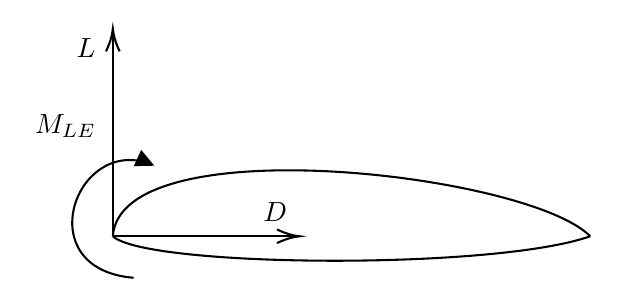
\begin{tikzpicture}[x=0.75pt,y=0.75pt,yscale=-1,xscale=1]
%uncomment if require: \path (0,300); %set diagram left start at 0, and has height of 300

%Curve Lines [id:da6282201102429681] 
\draw    (200,150) .. controls (203.67,97) and (400.18,119.75) .. (430,150) ;
%Curve Lines [id:da8779431608993546] 
\draw    (200,150) .. controls (216.34,165) and (383.51,166.41) .. (430,150) ;
%Straight Lines [id:da2590905789853304] 
\draw    (200,150) -- (200,52) ;
\draw [shift={(200,50)}, rotate = 90] [color={rgb, 255:red, 0; green, 0; blue, 0 }  ][line width=0.75]    (10.93,-3.29) .. controls (6.95,-1.4) and (3.31,-0.3) .. (0,0) .. controls (3.31,0.3) and (6.95,1.4) .. (10.93,3.29)   ;
%Straight Lines [id:da6275146811901227] 
\draw    (200,150) -- (288,150) ;
\draw [shift={(290,150)}, rotate = 180] [color={rgb, 255:red, 0; green, 0; blue, 0 }  ][line width=0.75]    (10.93,-3.29) .. controls (6.95,-1.4) and (3.31,-0.3) .. (0,0) .. controls (3.31,0.3) and (6.95,1.4) .. (10.93,3.29)   ;
%Curve Lines [id:da7637601528691369] 
\draw    (210,170) .. controls (159.47,165.85) and (181.66,102.38) .. (217.24,114.89) ;
\draw [shift={(220,116)}, rotate = 204.48] [fill={rgb, 255:red, 0; green, 0; blue, 0 }  ][line width=0.08]  [draw opacity=0] (8.93,-4.29) -- (0,0) -- (8.93,4.29) -- cycle    ;

% Text Node
\draw (181,53.4) node [anchor=north west][inner sep=0.75pt]    {$L$};
% Text Node
\draw (271,132.4) node [anchor=north west][inner sep=0.75pt]    {$D$};
% Text Node
\draw (161,90) node [anchor=north west][inner sep=0.75pt]    {$M_{LE}$};


\end{tikzpicture}

  \caption{前缘力矩}
  \label{fig:CenterOfPressure}
\end{figure}

一般规定,使得飞机抬头的力矩为正,使得飞机低头的力矩为负。
或者说,使得飞行迎角增大的力矩为正。

当气动力$N$和$A$减小时,$x_{cp}$增大。当气动力趋近于0时,
压心就移动到无穷远处了。


